
\FloatBarrier
\section{Система Лоренца} % _LOR_

\LinkRef{
  lor: ASAU-22, 23, 24, 25, 26.
  % ~/doc/tex/asau/asau22/atu/atu.tex
  % ~/doc/tex/asau/asau23/atu/atu.tex
  % ~/doc/tex/asau/asau24/atu/atu.tex
  APIR-2012. CSIT-2015. ISDMCI-2014, ISDMCI-2015.
  ITMM-2012, ITMM-2014, ITMM-2015, DSMP-2016
}


В качестве первой идентифицируемой хаотической системы рассмотрим классическую
систему Лоренца, динамика которой описывается системой
уравнений~\cite{moon_chaotic_vibr,anisch_nonlin_eff,chulichkcov_mm_ml_dyn}:
%
\begin{equation}
\begin{cases}
  \dot{x} = \sigma (y-x ) , \\
  \dot{y} = x (r-z) - y , \\
  \dot{z} = x y - b z .
\end{cases}
\label{atu:eq:lor}
\end{equation}

Наиболее ценным с точки зрения идентификации является параметр
$r$, определяющий как энергетическое состояние системы,
так и вид динамики системы.
Это подтверждают
расмотренные в дальнейшем физические обосноснования.
Для определённости зададим остальные параметры следующим классическим образом:
$b = 2.6666667$, $\sigma = 10$, если не будет явно указано обратное.


При малых значениях параметра $r$ система демонстрирует
затухающие колебания (рис.~\ref{atu:f:lor_attractor_fading}).

\begin{figure}[h!]
\begin{center}
  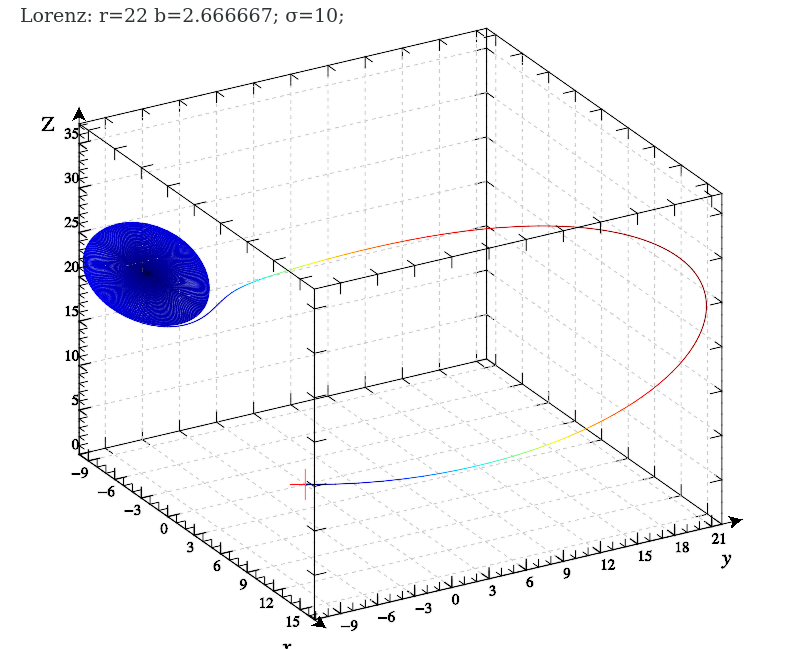
\includegraphics[width=0.49\textwidth]{p/cha/lor/lor0-p_xyz_r=022.png}
  \hfill
  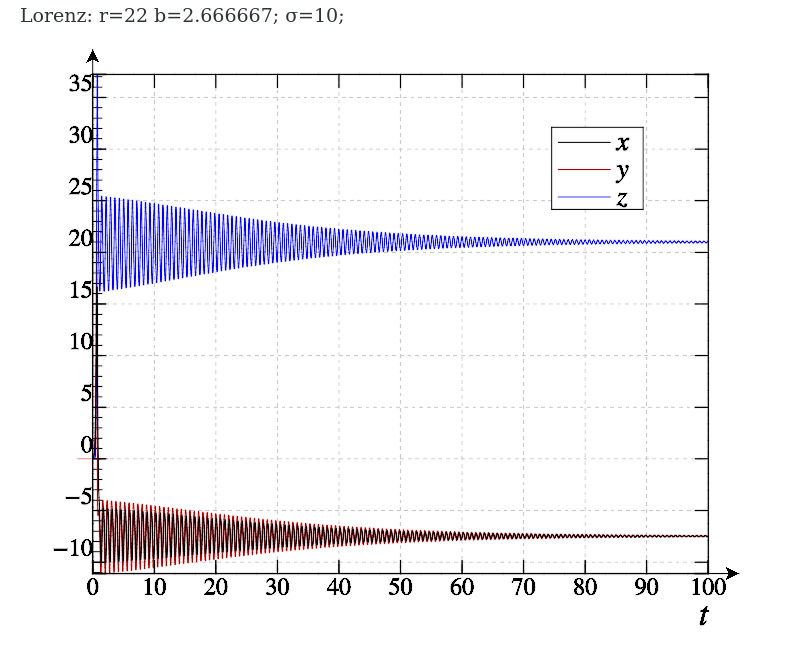
\includegraphics[width=0.49\textwidth]{p/cha/lor/lor0-p_t_r=022.png}
\end{center}
  \caption{Аттрактор и поведение переменных состояния системы Лоренца (\ref{atu:eq:lor}) в режиме затухающих колебаний ($r=22$)}
\label{atu:f:lor_attractor_fading}
\end{figure}

Далее,  в широком диапазоне значения параметра $r$
система проявляет хаотическую динамику. Помимо
этого, спектр данной системы в хаотическом режиме довольно широк
(рис.~\ref{atu:f:lor_attractor_phase_chaos28})
и не имеет доминирующих частот, что не характерно для многих систем
динамического хаоса.

\begin{figure}[h!]
\begin{center}
  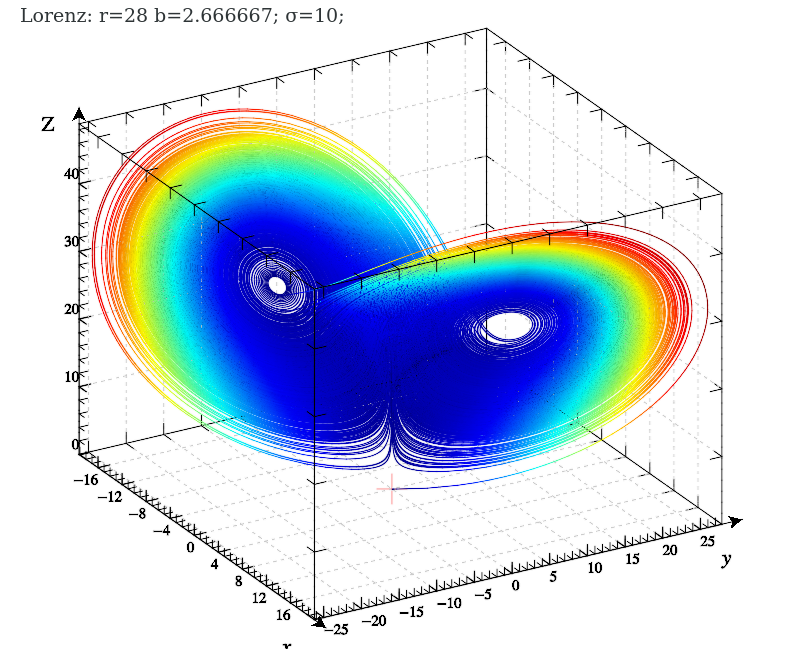
\includegraphics[width=0.49\textwidth]{p/cha/lor/lor0-p_xyz_r=028.png}
  \hfill
  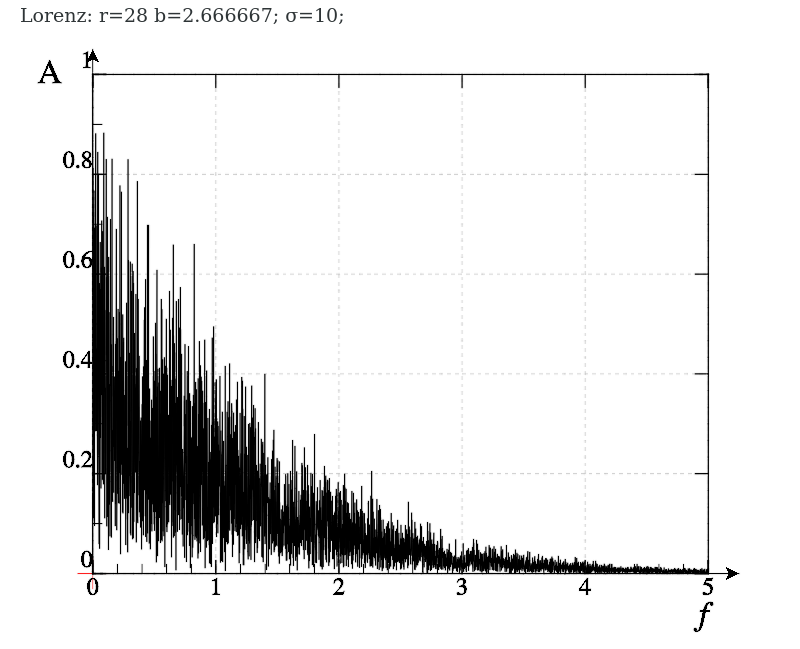
\includegraphics[width=0.49\textwidth]{p/cha/lor/lor0_fft-p_f_r=028.png}
\end{center}
  \caption{Аттрактор и спектр системы Лоренца (\ref{atu:eq:lor}) в хаотическом режиме ($r=28$)}
\label{atu:f:lor_attractor_phase_chaos28}
\end{figure}

При дальнейшем росте параметра $r$ динамика системы становится
сложно-периодической, с явно выраженным линейчатым спектром
(рис.~\ref{atu:f:lor_attractor_phase_200})

\begin{figure}[h!]
\begin{center}
  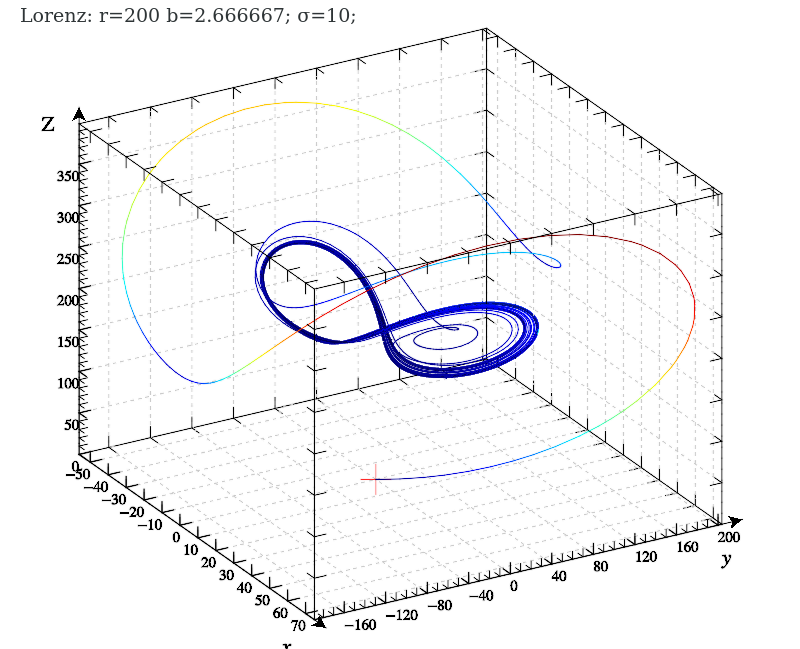
\includegraphics[width=0.49\textwidth]{p/cha/lor/lor0-p_xyz_r=200.png}
  \hfill
  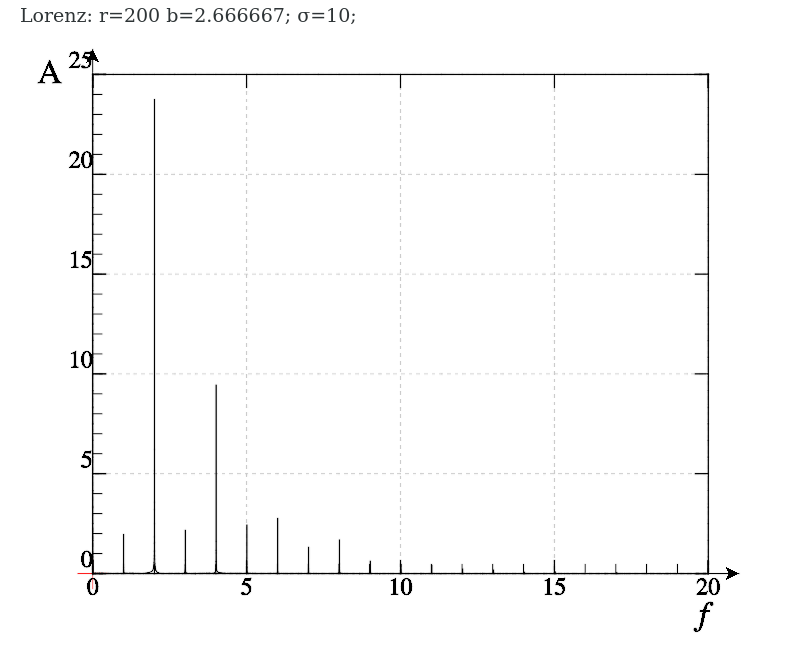
\includegraphics[width=0.49\textwidth]{p/cha/lor/lor0_fft-p_f_r=200.png}
\end{center}
  \caption{Аттрактор и спектр системы Лоренца (\ref{atu:eq:lor}) в сложно-периодическом режиме ($r=200$)}
\label{atu:f:lor_attractor_phase_200}
\end{figure}



Динамическая система Лоренца является одной из наиболее изученных
хаотических систем~\cite{neimark_stoch_chaos_vibro}.
При этом, существует множество физических систем, для
описания которых применима модель Лоренца. Это дает определённые основания
предполагать, что синтез критерия идентификации, основанного на физических
принципах, для данной системы будет успешным.


Для синтеза критерия идентификации параметра $r$ системы (\ref{atu:eq:lor}), рассмотрим
набор физических систем, для моделирования которых применяется система
Лоренца.

Исторически первой такой системой, рассмотренной самим Лоренцом, является
задача о тепловой конвекции жидкости в плоском слое. Исходная система
уравнений гидродинамики имеет вид:
%
%
\begin{equation}
\begin{cases}
  \pd{\vec{v}}{t} + ( \vec{v} \nabla ) \vec{v} = - \frac{\nabla p}{\rho} + \nu \Delta \vec{v} + \vec{g}, \\
  \pd{\rho}{t} + \nabla ( \rho \vec{v} ) = 0 , \\
  \pd{T}{t} +\nabla ( T \vec{v} ) = \chi \Delta T , \\
  \rho = \rho_0 \left( 1 - \gamma (T - T_0) \right) .
\end{cases}
\label{atu:eq:lor_gidro}
\end{equation}
%
где
$\vec{v} $   -- поле скоростей,
$T$ -- поле температуры,
$T_0$ и $T_0+\Delta T$   -- температуры на верхней и нижней границе соответственно,
$\rho$ и $p$ -- поля плотности и давления,
$g$ -- ускорение свободного падения,
$\nu$, $\chi$, $\gamma$  -- коэффициенты кинематической вязкости, температуропроводности и
теплового расширения соответственно.

При приближении системы (\ref{atu:eq:lor_gidro}) к виду (\ref{atu:eq:lor}),
переменные и параметры системы
Лоренца определяются следующим образом: $x$ задаёт скорость вращения валов
течения, $y$, $z$ -- соответствуют распределению температуры по горизонтали и
вертикали.
$\sigma$   -- число Прандтля (отношение коэффициентов кинематической вязкости и
температуропроводности). Параметр $b$ определяет отношения размеров ячейки.
$r$ -- (идентифицируемый параметр) -- приведённое число Релея, определяющее
энергетические параметры конвекционного течения.

Из трёх переменных состояния проще всего наблюдению поддаётся переменная
$x$. С другой стороны, так как параметр $r$ определяет энергетические
соотношения в системе, то и критерий качества должен представлять собой
квадратичную форму от $x$, причём усреднённую на интервале времени,
существенно большем, чем характерное время оборота жидкостного вала.

Другой системой, для моделирования которой применяется система Лоренца --
это модель одномодового лазера. В этой модели переменной $x$ соответствует
амплитуда поля в резонаторе, $y$ -- поляризации, $z$ -- инверсии заселённости
квантовых уровней активной среды. Параметры $\sigma$ и $b$
определяются отношениями коэффициентов релаксации, а искомый параметр $r$
определяется удельной мощностью накачки.

Как и в случае гидродинамической системы, наиболее просто наблюдаемым
параметром является $x$ -- именно он определяет выходную интенсивность. И
опять же, по аналогии -- идентифицируемый параметр $r$ определяет энергетику
системы. При переходе от амплитуды к мощности совершенно аналогично
следует использовать квадратичную зависимость.

Также система (\ref{atu:eq:lor}) применима для
моделирования конвекции жидкости в замкнутом подогреваемом петле,
динамики водяного колеса, осцилляторе с трением и других~\cite{kuznetsov_dyn_chaos}.

Таким образом, в первую очередь следует проверить применимость
критерия вида $q_{x^2}$. Тем не менее, проверим все
критерии данного вида, применимые к данной системе.
На рис.~\ref{atu:f:lor_q} приведены исследуемые зависимости
$q_{*}(r)$, полученные путём моделирования динамики
системы \ref{atu:eq:lor} для различных значений параметра~$r$,
при усреднении на значительном временном интервале $\tau_q=500$.


\begin{figure}[h!]
  \centerline{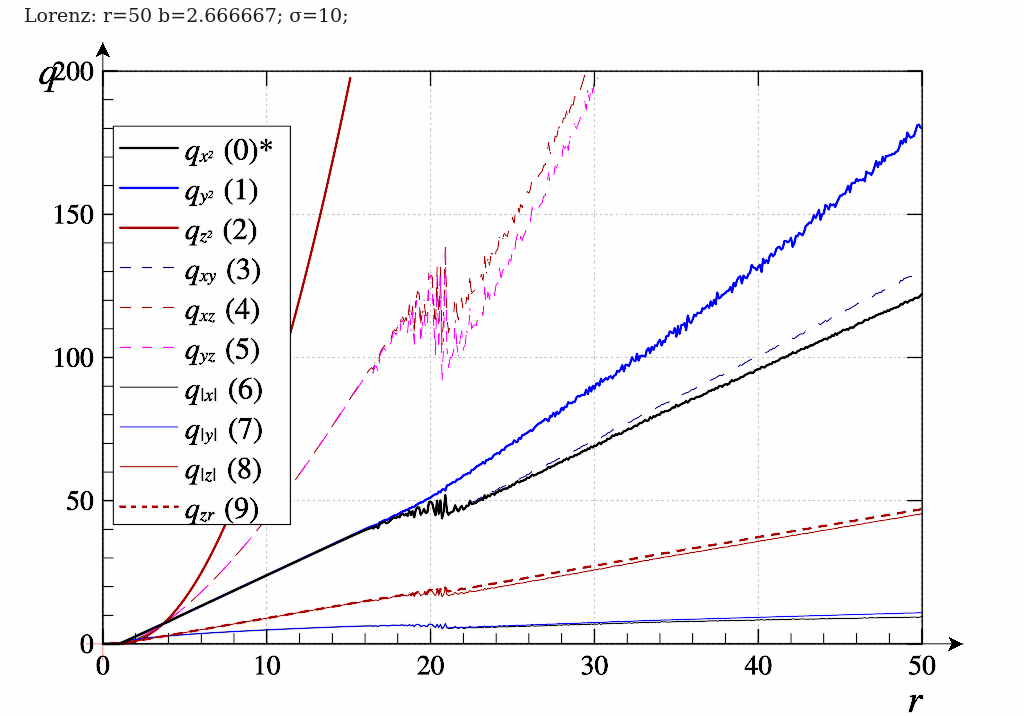
\includegraphics[width=0.7\textwidth]{p/cha/lor/lor_q-p_q_r.png} }
  \caption{Рассматриваемые критерии для системы Лоренца}
  \label{atu:f:lor_q}
\end{figure}

Анализ графиков позволяет сделать вывод, что практически все
рассмотренные виды критериев должны позволять построить
работоспособную систему идентификации. При этом,
большая часть графиков, в том числе и изначально
предложенный $q_{x^2}$, теряют монотонность
при переходе от режима затухающих колебаний к хаотическому,
что может помешать процессу идентификации вблизи этой точки.
Тем не менее, режим затухающих колебаний не представляет
практического интереса, и этим недостатком можно пренебречь.
Этого недостатка лишён критерий $q_{y^2}$, однако,
в рассматриваемых физических задачах значение
$y(t)$ наблюдать сложнее. К тому же, в первом приближении
зависимость $q_{x^2}(r)$ -- линейная, а
$q_{y^2}(r) \sim \sqrt{r}$.
Спектры же сигналов $x(t)$, $y(t)$ и $z(t)$
имеют практически одинаковую структуру.
Поэтому, в дальнейших исследованиях ограничимся
критериями
$q_{x^2}$ и
$q_{y^2}^2$.

Следующая зависимость, необходимая для синтеза
системы идентификации -- $ \sigma_q(\tau_q) $
или же  $ \sigma_q(a_q) $ -- соотношение между
временем оценивания $\tau_q$ и среднеквадратичной
ошибкой измерения критерия.
Для моделирования непосредственных погрешностей измерения величин
$x(t)$ и $y(t)$ использовался шум с нормальным распределением
и параметрами $\sigma_w=0.5$ и $\tau_w=0.05$.
Для оценивания требуемой зависимости, для каждого
значения $\tau_q$ из заданного диапазона
проводилось $N=200$ процессов моделирования динамики системы,
и в случайный момент (достаточно далеко отстоящий от точки $t=0$ для исключения краевых эффектов)
проводилось измерение и запоминание выбранного критерия.
При этом, для усреднения величины $q$ использовалось 2 метода:
простейший линейный, вида (\ref{atu:eq:qlin}), и скользящее среднее.
Полученные зависимости, обозначенные соответственно
$\sigma_{ql}$ и $\sigma_{qa}$, представлены на
рис.~\ref{atu:f:lor_qy2_tau} и~\ref{atu:f:lor_qx2_tau}.


\begin{figure}[h!]
\begin{center}
  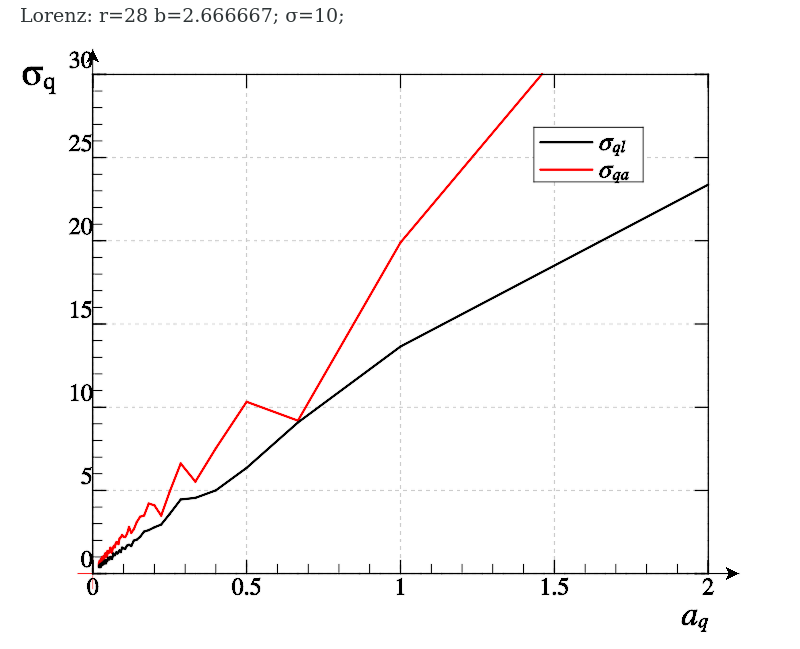
\includegraphics[width=0.49\textwidth]{p/cha/lor/lor_q_tau-p_aq_sd.png}
  \hfill
  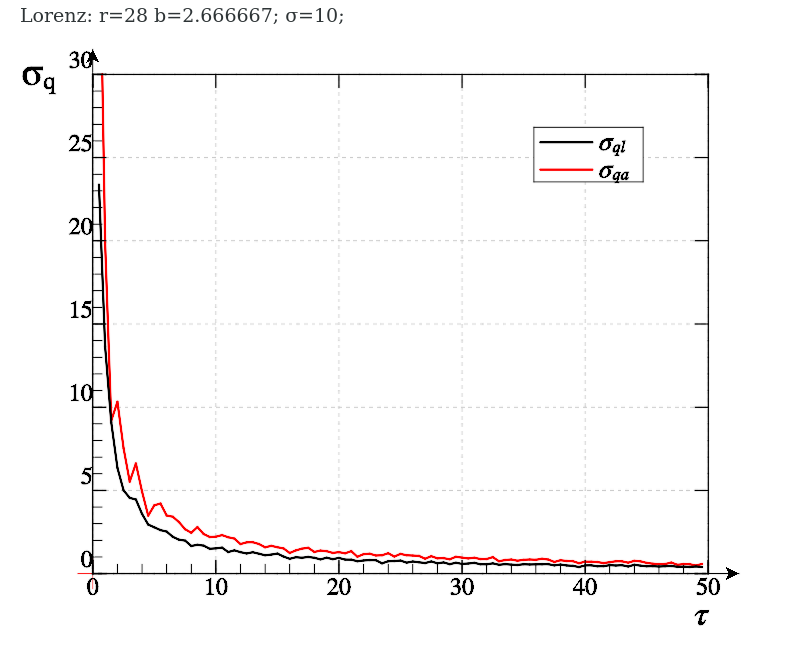
\includegraphics[width=0.49\textwidth]{p/cha/lor/lor_q_tau-p_tau_sd.png}
\end{center}
  \caption{Зависимости $\sigma_{q}(a_q)$ и $\sigma_{q}(\tau_q)$ для системы Лоренца, критерий  $q_{y^2}$}
\label{atu:f:lor_qy2_tau}
\end{figure}


\begin{figure}[h!]
\begin{center}
  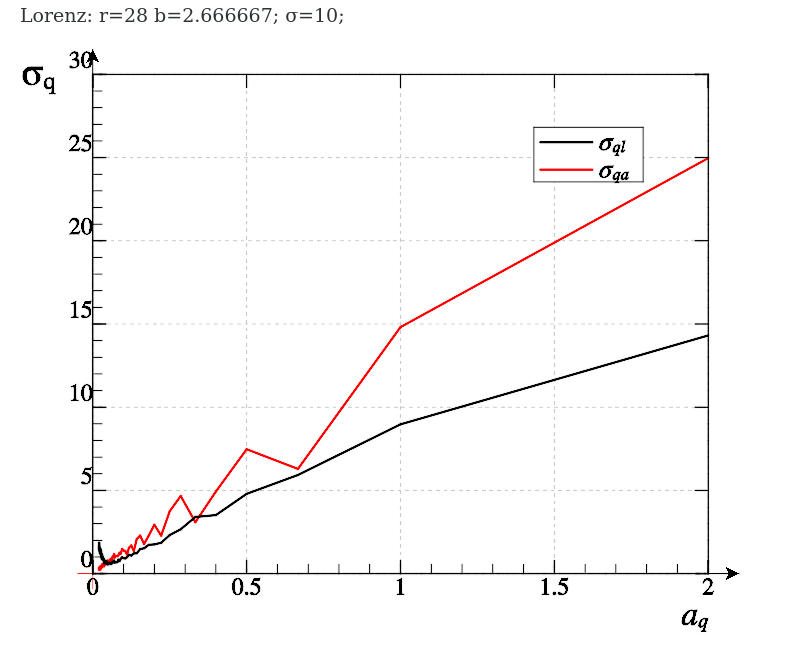
\includegraphics[width=0.49\textwidth]{p/cha/lor/lor_qx2_tau-p_aq_sd.png}
  \hfill
  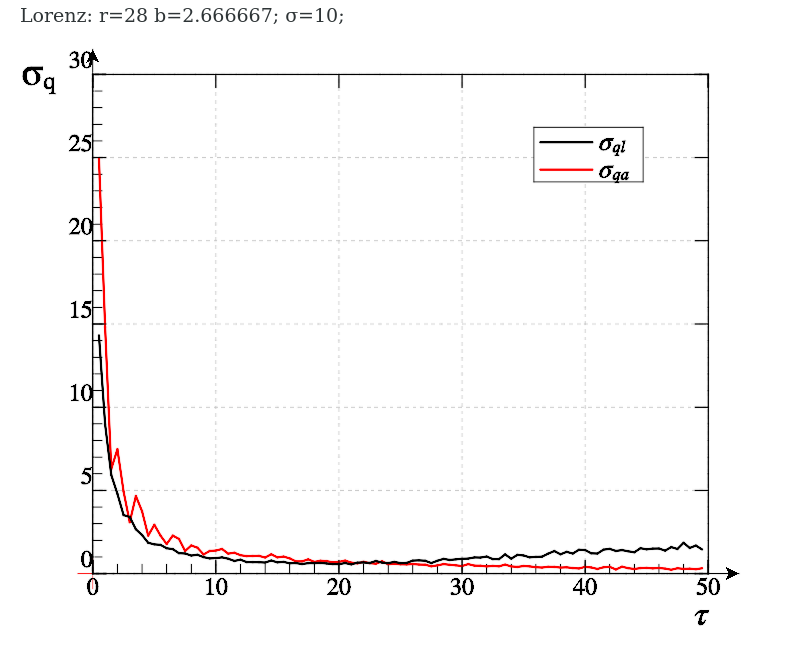
\includegraphics[width=0.49\textwidth]{p/cha/lor/lor_qx2_tau-p_tau_sd.png}
\end{center}
  \caption{Зависимости $\sigma_{q}(a_q)$ и $\sigma_{q}(\tau_q)$ для системы Лоренца, критерий $q_{x^2}$}
\label{atu:f:lor_qx2_tau}
\end{figure}

Анализ полученных зависимостей позволяет сделать
несколько выводов. Прежде всего, для рассматриваемой системы
результат усреднения с помощью значительно более затратного
в реализации метода скользящего среднего практически везде
уступает более простому методу. Таким образом,
при реализации методов идентификации в условиях с ограниченным ресурсами,
например на микроконтроллерной платформе в реальном времени,
нет смысла реализовывать ресурсоёмкоё скользящее среднее.
Далее, сам вид зависимости оказался достаточно простым:
$ \sigma_q \sim q a_q $ или же
$ \frac{\sigma_q \tau_q}{q} \approx \mathrm{const}$.

В соответствии с полученными данными, и следуея
предложениям~(\ref{atu:eq:po_t_sign}) и~(\ref{atu:eq:po_t_sin}),
определим тестовую задачу следующим образом:
\[
  p(t) \in [20, 60],
\]
%
\begin{equation}
  r_o(t) = p_o(t) = p_0 +  U_{p} \sign \sin( \omega_{p} t ),
  \label{atu:eq:lor_po_t_sign}
\end{equation}
%
%
\begin{equation}
  r_o(t) = p_o(t) = p_0 +  U_{p} \sin( \omega_{p} t ),
  \label{atu:eq:lor_po_t_sin}
\end{equation}
%
где:
$p_0 = 37$, $U_p=12$, $\omega_p=0.09$.

Для сравнения были выбраны три группы мультимодельных методов идентификации:
qAuv5.3r.$q_{x^2}$,
qAuv5.3r.$q_{y^2}$ и
FAlv5.3z.$q_{x^2}$. Символ ``A'' на второй позиции каждого из
обозначений~(см.~стр.~\pageref{atu:id_classification})
обозначает, что проверяются
все возможные способы определения $p_{id}$,
а количество агентов и способ их группировки (5.3) были выбраны
одинаковыми для корректного сравенения различных походов.


На рис.~(\ref{atu:f:lor_id_qAuv5.3r.q_x2_sign}) представлены результаты
методом qAuv5.3r.$q_{x^2}$, при этом на левом графике представлена
динамика перемещения каждой из подвижных моделей,
а на правом -- 4 споcоба определения $p_{id}(t)$:
$p_{ge}$, $p_{le}$, $p_{ee}$ и $p_{xe}$.
В первую очередь, следует отметить общую работоспособность
методов, и правильную динамику каждой из моделей.
Сравнивая результаты различных способов определения
$p_{id}$ как визуально, так и численно, можно сделать
вывод, что худшие результаты демонстрирует $p_{ee}$.
Этого и следовало ожидать, так как это подход, в первую очередь,
был предназначен для методов идентификации, использующих
функцию качества для определения $p_e$.
Также, совершенно ожидаемо, лудшие результаты продемонстирировал
подход $p_{xe}$. Также, при искусственных ограничения
$v_f=0$ и $q_\gamma=0.1$ были получены величины,
характеризующие качество идентификации для неподвижных агентов:
$\overline{e}_{bm}=9.85$
и
$\overline{e}_{ba}=7.09$, что свидетельствует
о оправданности как перемещения агентов,
так и использвании величин $p_e$ для определения $p_{id}$.



\begin{figure}[h!]
  \centerline{
    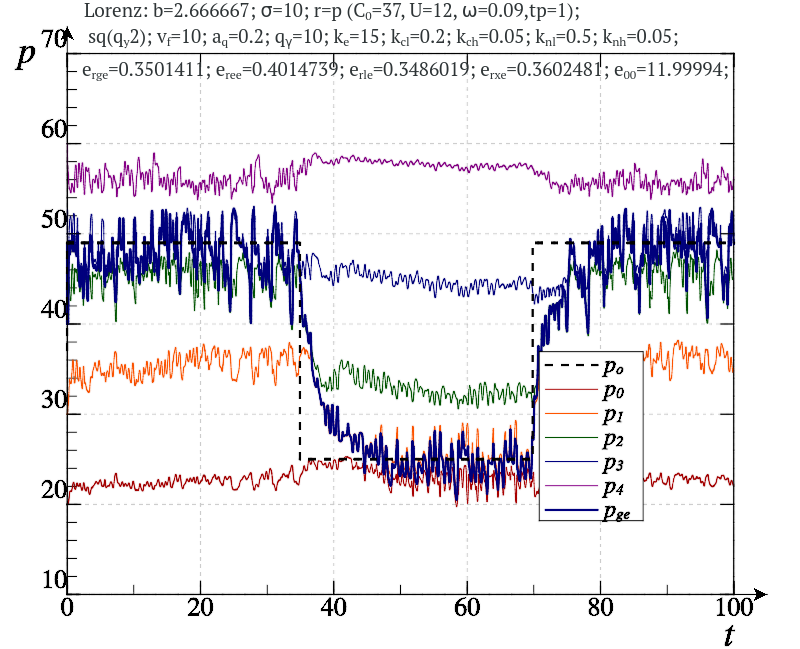
\includegraphics[width=0.49\textwidth]{p/cha/lor/qAuv5.3r/lor_qAuv5_3r_qy2-p_t_pi_sign.png}
    \hfill
    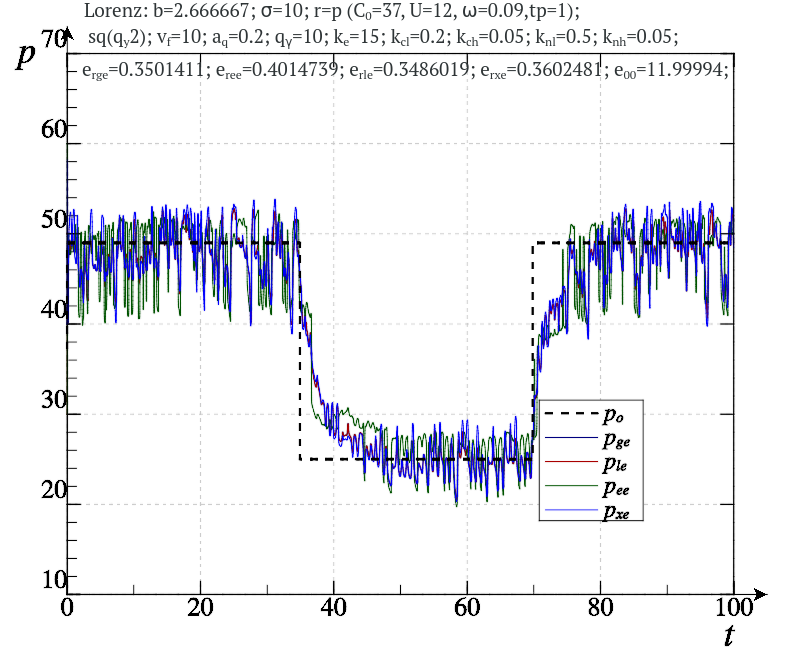
\includegraphics[width=0.49\textwidth]{p/cha/lor/qAuv5.3r/lor_qAuv5_3r_qy2-p_t_pz_sign.png}
  }
  \caption{Процесс идентификации параметра ``$r$'' системы Лоренца методом qAuv5.3r.$q_{x^2}$ при условии~(\ref{atu:eq:lor_po_t_sign})}
  \label{atu:f:lor_id_qAuv5.3r.q_x2_sign}
\end{figure}


На рис.~(\ref{atu:f:lor_id_qAuv5.3r.q_x2_sin}) представлены аналогичные результаты,
но при условии плавного изменение значения параметра объекта. Как и следовало ожидать,
как абсолютные, так и относительные значения ошибок идентификации в данном случае заметно
меньше, при сохранении общей картины.
При этом
$\overline{e}_{bm}=7.80$
и
$\overline{e}_{ba}=5.24$.


\begin{figure}[h!]
  \centerline{
    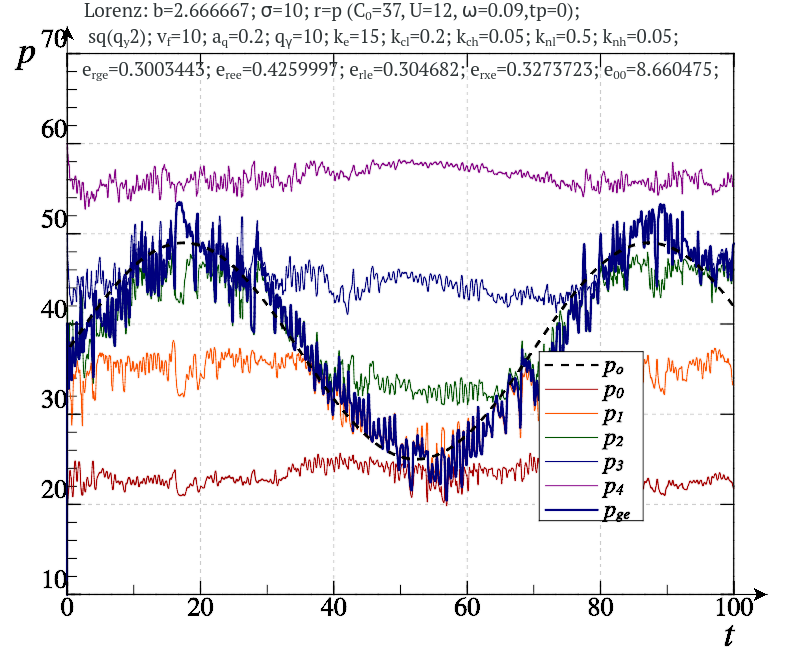
\includegraphics[width=0.49\textwidth]{p/cha/lor/qAuv5.3r/lor_qAuv5_3r_qy2-p_t_pi_sin.png}
    \hfill
    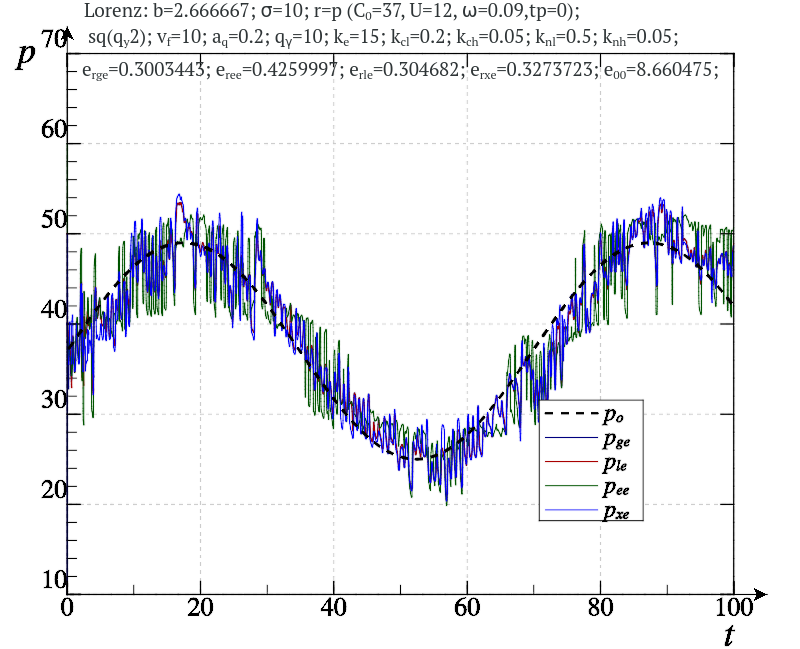
\includegraphics[width=0.49\textwidth]{p/cha/lor/qAuv5.3r/lor_qAuv5_3r_qy2-p_t_pz_sin.png}
  }
  \caption{Процесс идентификации параметра ``$r$'' системы Лоренца методом qAuv5.3r.$q_{x^2}$ при условии~(\ref{atu:eq:lor_po_t_sin})}
  \label{atu:f:lor_id_qAuv5.3r.q_x2_sin}
\end{figure}


На рис.~(\ref{atu:f:lor_id_qAuv5.3r.q_y2_sign}) представлены результаты
полученные методом qAuv5.3r.$q_{y^2}$,
отличающего от предыдущего только видом использованного критерия
и немного-по другому настроенными параметрами самой системы идентификации,
для отражения свойств данного критерия.
При этом
$\overline{e}_{bm}=10.85$
и
$\overline{e}_{ba}=7.73$.

\begin{figure}[h!]
  \centerline{
    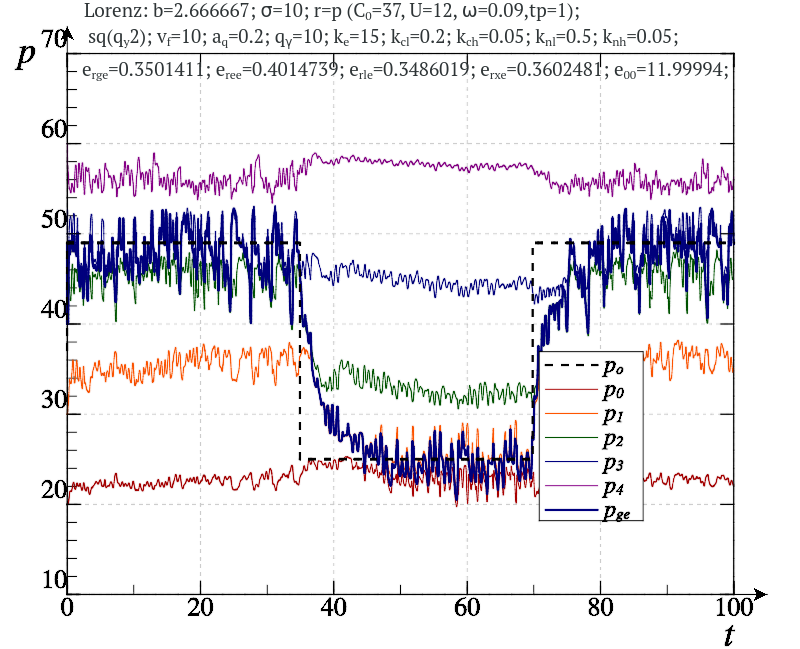
\includegraphics[width=0.49\textwidth]{p/cha/lor/qAuv5.3r/lor_qAuv5_3r_qy2-p_t_pi_sign.png}
    \hfill
    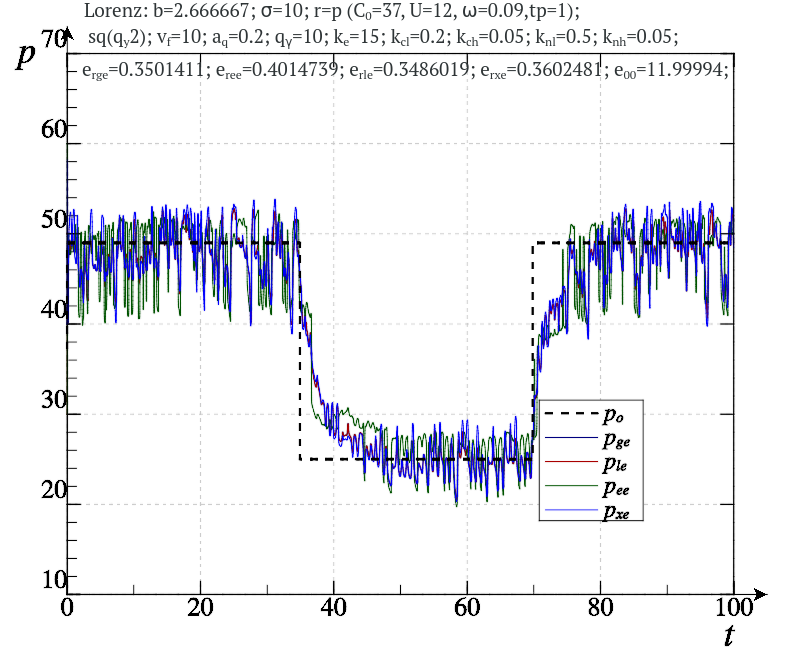
\includegraphics[width=0.49\textwidth]{p/cha/lor/qAuv5.3r/lor_qAuv5_3r_qy2-p_t_pz_sign.png}
  }
  \caption{Процесс идентификации параметра ``$r$'' системы Лоренца методом qAuv5.3r.$q_{y^2}$ при условии~(\ref{atu:eq:lor_po_t_sign})}
  \label{atu:f:lor_id_qAuv5.3r.q_y2_sign}
\end{figure}


На рис.~(\ref{atu:f:lor_id_qAuv5.3r.q_y2_sin}) представлены аналогичные результаты,
только при условии (\ref{atu:eq:lor_po_t_sin}).
При этом
$\overline{e}_{bm}=8.09$
и
$\overline{e}_{ba}=5.46$.


\begin{figure}[h!]
  \centerline{
    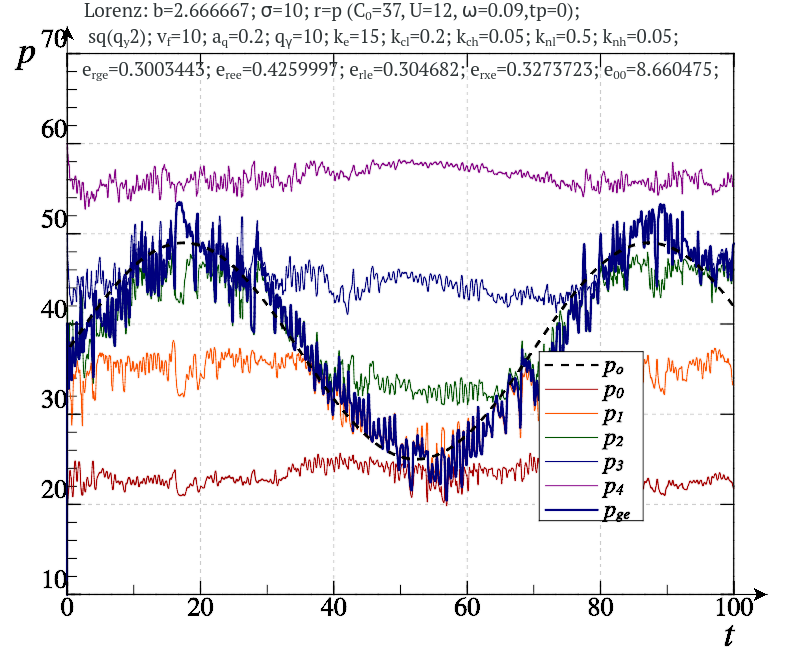
\includegraphics[width=0.49\textwidth]{p/cha/lor/qAuv5.3r/lor_qAuv5_3r_qy2-p_t_pi_sin.png}
    \hfill
    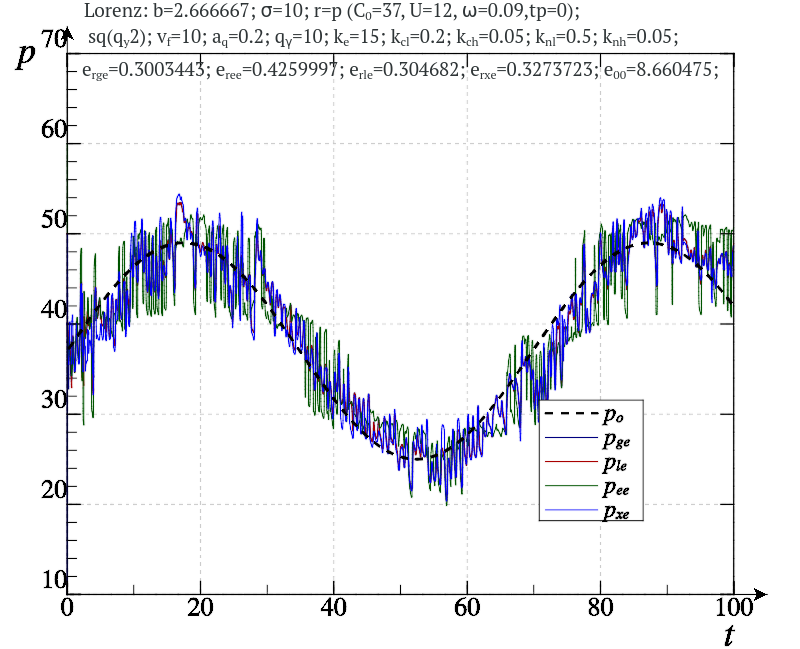
\includegraphics[width=0.49\textwidth]{p/cha/lor/qAuv5.3r/lor_qAuv5_3r_qy2-p_t_pz_sin.png}
  }
  \caption{Процесс идентификации параметра ``$r$'' системы Лоренца методом qAuv5.3r.$q_{x^2}$ при условии~(\ref{atu:eq:lor_po_t_sin})}
  \label{atu:f:lor_id_qAuv5.3r.q_y2_sin}
\end{figure}

Сравнивая результаты, представленные на рис.~(\ref{atu:f:lor_id_qAuv5.3r.q_x2_sign})--\ref{atu:f:lor_id_qAuv5.3r.q_y2_sin}
можно сделать следующие выводы:

\begin{itemize}

  \item
    Динамика систем идентификации при использовании критериев $q_{x^2}$ и $q_{y^2}$
    практически совпадает.

  \item
    Применение критерия  $q_{y^2}$ в данном конкретном случае позволяет
    меньшую ошибку идентификации, но на настолько,
    чтобы можно было говорить о существенной разнице.

  \item
    Во всех рассмотренных случаях оправданными были и применение нескольких агентов,
    и их смещение в процессе поиска, и аппроскимация с помощью $p_e$
    каждого из агентов.

\end{itemize}

Рассмотри процесс идентификации этой же системы, при тех же условиях,
но семейством методов, основанных на применении функции качества,
а именно FAlv5.3z.$q_{x^2}$

Процесс идентификации при условии~(\ref{atu:eq:lor_po_t_sign})
представлен на рис.~(\ref{atu:f:lor_id_FAlv5.3z.q_x2_sign}).
В первую очередь следует отметить большую подвижность
агентов, вплоть до искуственного ограничения подвижности
большей части моделей. С одной стороны, это несколько уменьшает
быстродействие системы при резких изменениях параметра,
с другой -- обеспечивает достаточное смещение ``дальних'' агентов,
что, в какой-то мере, компенсирует возможные ошибки в настройке системы.
Величина $\overline{e}_{bm}=10.84$ имеет примерно такое же значение,
как и предудущих случаях,
а $\overline{e}_{ba}$ в данных условиях не применимо.

\begin{figure}[h!]
  \centerline{
    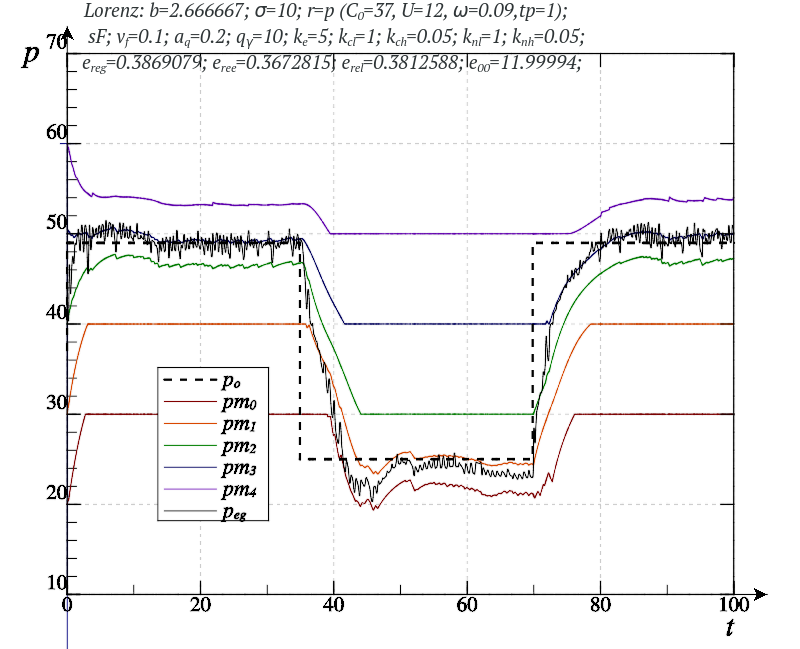
\includegraphics[width=0.49\textwidth]{p/cha/lor/FAlv5.3z/lor_FAlv5_3z_qx2-pl_n_sign.png}
    \hfill
    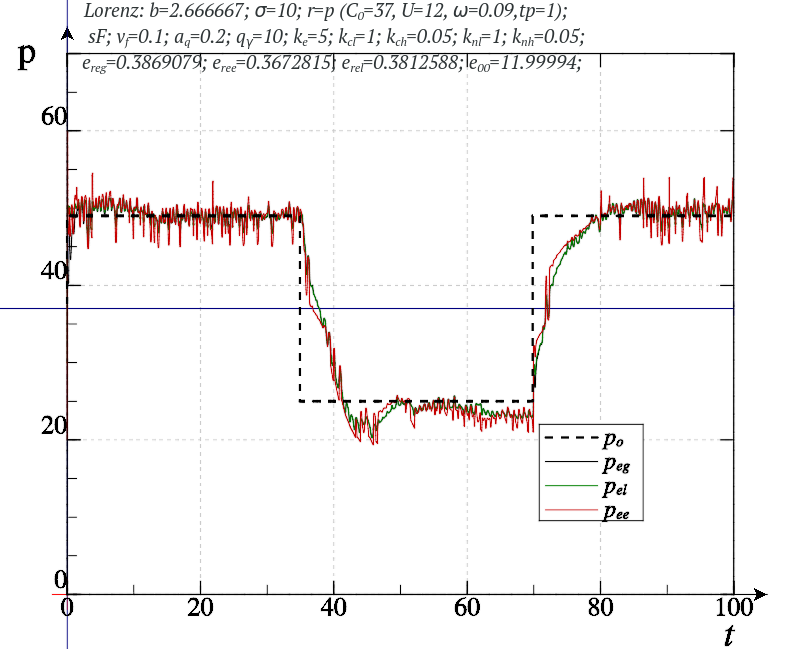
\includegraphics[width=0.49\textwidth]{p/cha/lor/FAlv5.3z/lor_FAlv5_3z_qx2-p_p_sign.png}
  }
  \caption{Процесс идентификации параметра ``$r$'' системы Лоренца методом FAlv5.3z.$q_{x^2}$ при условии~(\ref{atu:eq:lor_po_t_sign})}
  \label{atu:f:lor_id_FAlv5.3z.q_x2_sign}
\end{figure}

На рис.~(\ref{atu:f:lor_id_FAlv5.3z.q_x2_sin})
процесс идентификации при условии~(\ref{atu:eq:lor_po_t_sin}).
Величина $\overline{e}_{bm}=7.95$ не выбивается из общего ряда,
и общая катрина имеет ожидаемый вид.

\begin{figure}[h!]
  \centerline{
    \includegraphics[width=0.49\textwidth]{p/cha/lor/FAlv5.3z/lor_FAlv5_3z_qx2-pl_n_sin.png}
    \hfill
    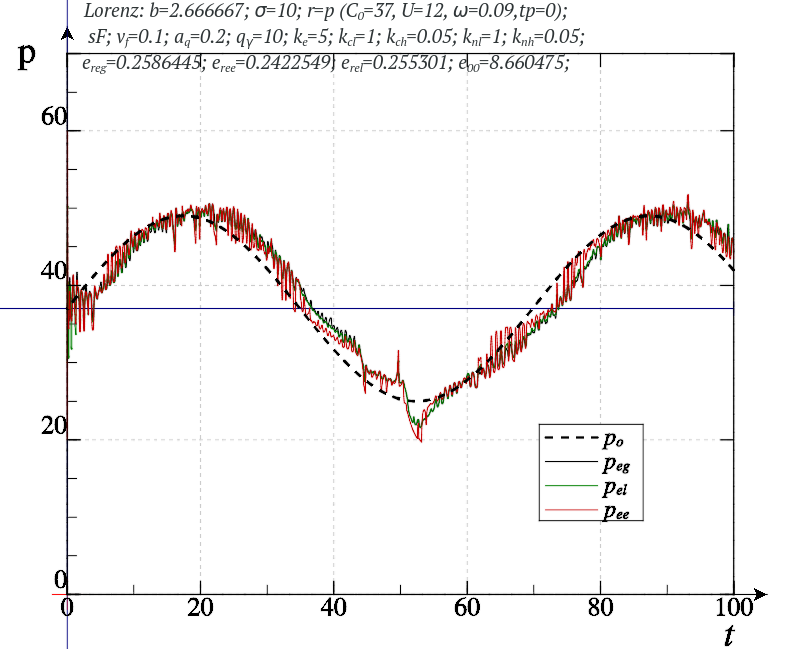
\includegraphics[width=0.49\textwidth]{p/cha/lor/FAlv5.3z/lor_FAlv5_3z_qx2-p_p_sin.png}
  }
  \caption{Процесс идентификации параметра ``$r$'' системы Лоренца методом FAlv5.3z.$q_{x^2}$ при условии~(\ref{atu:eq:lor_po_t_sin})}
  \label{atu:f:lor_id_FAlv5.3z.q_x2_sin}
\end{figure}


Рассмотрим влияние параметров системы идентифкации на
процесс идентификации и, следовательно, на ёё качество.
Для этого будем варьировать каждый из существенных
параметров и строить зависимости $\overline{e}_{r*}$
для каждого из рассмотренных методов.

В первую очередь рассмотрим влияение параметра
$a_q$, определяющего характрерное время усреднения.

На рис.~(\ref{atu:f:lor_a_q_qAuv5.3r.q_x2}) представлены зависимости
усреднённых ошибок идентификации системы Лоренца от $a_q$ при использованни метода qAuv5.3r.$q_{x^2}$.
Достаточно очевидно, что форма кривых с явным экстремумом обусловлена
влияниями противобоствующих факторов. При больших значениях $a_q$,
и, следовательно, малом времени усреднения $\tau_q$,
слишком сильно влияние хаотической динамики, что бы можно было бы
проводить успешную идентфикацию. С другой стороны,
при слишком малых значениях $a_q$, время оценивание критерия настолько большое,
что система идентификации не успевает отслеживать изменение параметра.
Этот тезис подтверждается тем фактом, что при более плавном изменении параметра
(\ref{atu:eq:lor_po_t_sin})
минимум ошибок достигается при меньших значениях $a_q$.

\begin{figure}[h!]
  \centerline{
    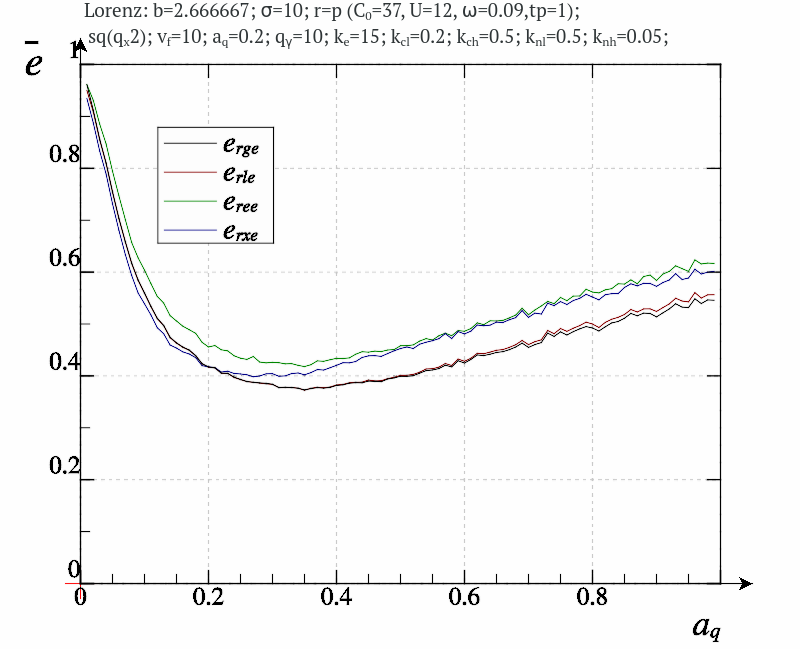
\includegraphics[width=0.49\textwidth]{p/cha/lor/qAuv5.3r/lor_qAuv5_3r_qx2-p_a_q_e_sign.png}
    \hfill
    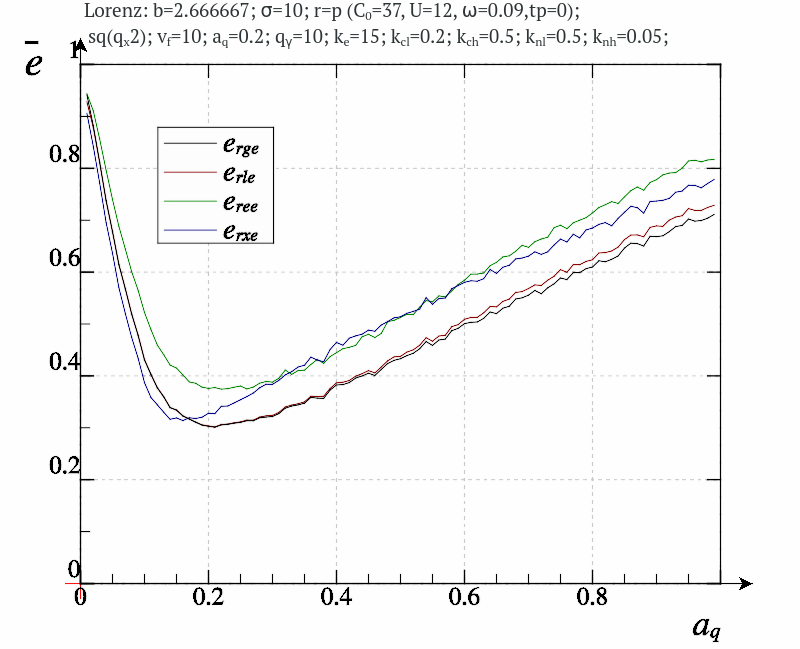
\includegraphics[width=0.49\textwidth]{p/cha/lor/qAuv5.3r/lor_qAuv5_3r_qx2-p_a_q_e_sin.png}
  }
  \caption{Зависимости $\overline{e}_{r*}(a_q)$ при идентификации системы Лоренца методом qAuv5.3r.$q_{x^2}$
   при~(\ref{atu:eq:lor_po_t_sign}) и (\ref{atu:eq:lor_po_t_sin})}
  \label{atu:f:lor_a_q_qAuv5.3r.q_x2}
\end{figure}


На рис.~(\ref{atu:f:lor_a_q_qAuv5.3r.q_y2}) представлены зависимости
усреднённых ошибок идентификации системы Лоренца при использованни метода qAuv5.3r.$q_{y^2}$.
Здесь ситуация существенно изменяется но сравнениею с предыдущим случаем.
Положения экстремумов практически не изменились, но
при больших значениях $a_q$ начинает наблюдаться полное нарушение
процесса поиска. Таким образом, несмотря на то,
что в наилудших условиях критерий $q_{y^2}$ обеспечивает меньшую
ошибку идентификации, диапазон его примеримости меньше. С учётом
того, момент нарушения поиска зависит и от формы $p_o(t)$,
а она в реальных задачах заранее не известна, использование этого критерия может
не быть оправданным.

\begin{figure}[h!]
  \centerline{
    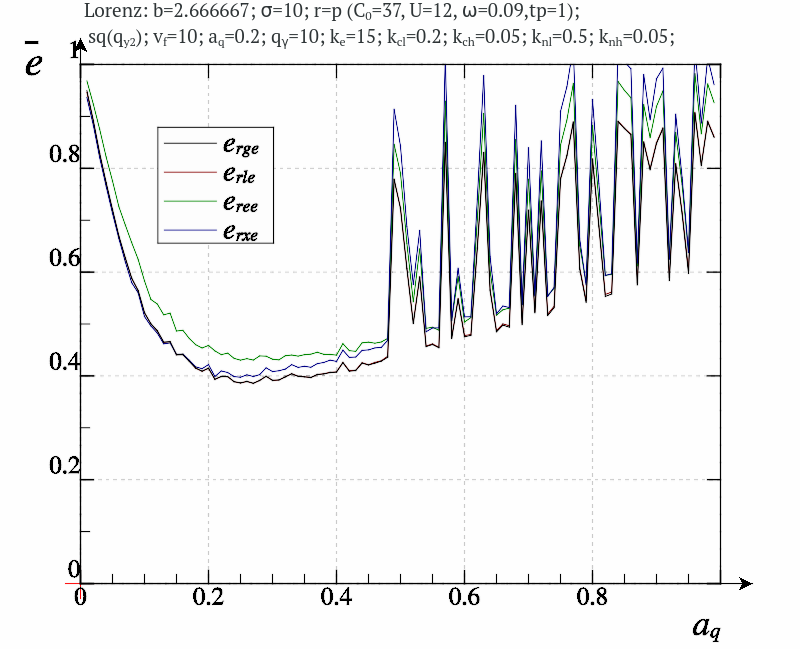
\includegraphics[width=0.49\textwidth]{p/cha/lor/qAuv5.3r/lor_qAuv5_3r_qy2-p_a_q_e_sign.png}
    \hfill
    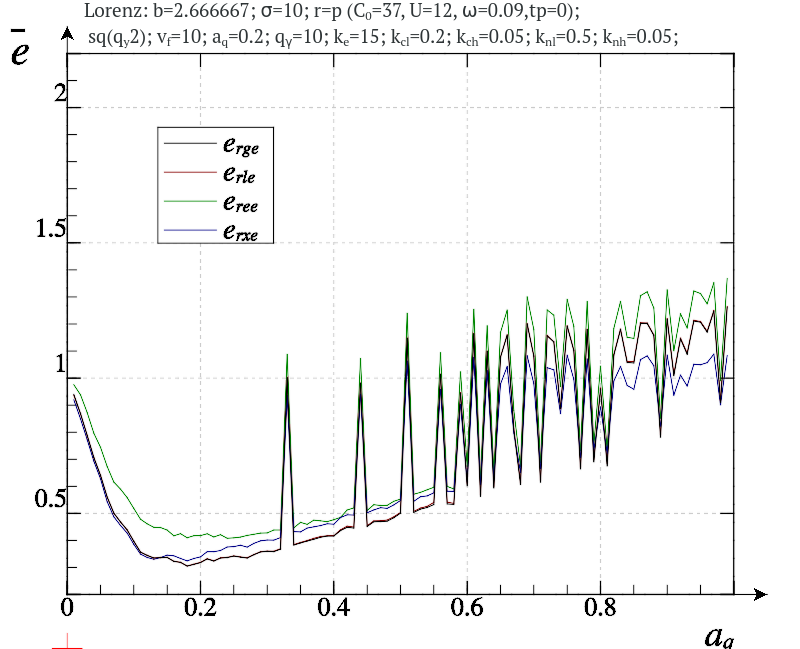
\includegraphics[width=0.49\textwidth]{p/cha/lor/qAuv5.3r/lor_qAuv5_3r_qy2-p_a_q_e_sin.png}
  }
  \caption{Зависимости $\overline{e}_{r*}(a_q)$ при идентификации системы Лоренца методом qAuv5.3r.$q_{y^2}$
   при~(\ref{atu:eq:lor_po_t_sign}) и (\ref{atu:eq:lor_po_t_sin})}
  \label{atu:f:lor_a_q_qAuv5.3r.q_y2}
\end{figure}


На рис.~(\ref{atu:f:lor_a_q_FAlv5.3z.q_x2}) представлены зависимости
усреднённых ошибок идентификации системы Лоренца при использованни метода FAlv5.3z.$q_{x^2}$.
Как характер зависимостей, так и положение экстремумов аналогичны
случаю при использовании метода  qAuv5.3r.$q_{x^2}$,
хотя определённые различия наблюдаются. Тем не менее,
можно сделать вывод, что как оптимальные значения величины $a_q$,
так и диапазон применимости в первую очередь определяется
критерием и динамикой изменения параметра, и уже во вторую очередь --
конкретным методом.


\begin{figure}[h!]
  \centerline{
    \includegraphics[width=0.49\textwidth]{p/cha/lor/FAlv5.3z/lor_FAlv5_3z_qx2-p_a_q_e_sign.png}
    \hfill
    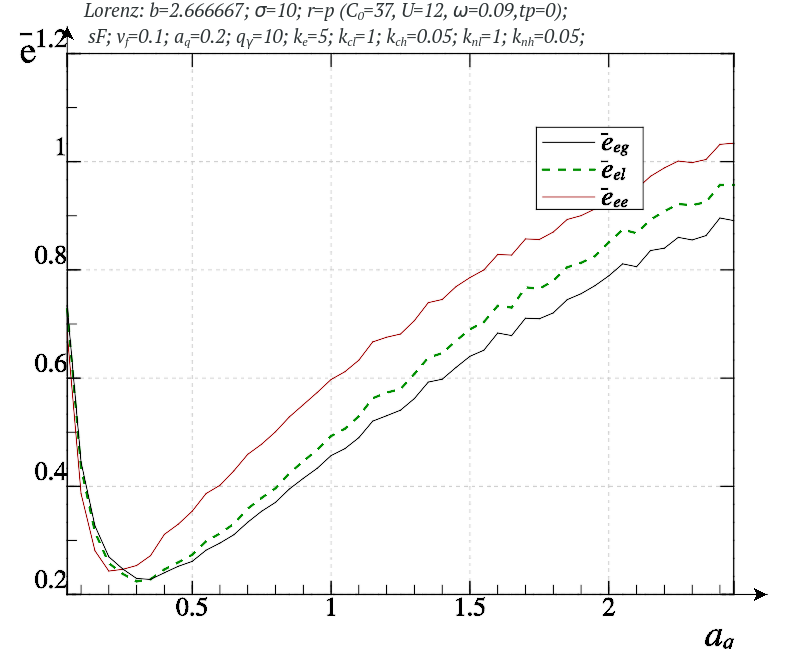
\includegraphics[width=0.49\textwidth]{p/cha/lor/FAlv5.3z/lor_FAlv5_3z_qx2-p_a_q_e_sin.png}
  }
  \caption{Зависимости $\overline{e}_{r*}(a_q)$ при идентификации системы Лоренца методом FAlv5.3z.$q_{x^2}$
   при~(\ref{atu:eq:lor_po_t_sign}) и (\ref{atu:eq:lor_po_t_sin})}
  \label{atu:f:lor_a_q_FAlv5.3z.q_x2}
\end{figure}


Слкдующий важные параметр -- масштаб фаекции качества $q_\gamma$.
В первую очередь он должен влиять на методы,
котоные используют величину $F$ в процессе поиска.
С другой стороны, методы, использующие только критерий для
определения $p_e$, тоже используют  $q_\gamma$ в процессе
определения $p_{id}$.

На рис.~(\ref{atu:f:lor_qg_qAuv5.3r.q_x2}) представлены зависимости
усреднённых ошибок идентификации системы Лоренца от $q_\gamma$ при использованни метода qAuv5.3r.$q_{x^2}$.
Как и предполагалось, зависимости достаточно слабые, за исключением $\overline{e}_{rge}$,
для которой большие величины масштаба обозначают малую чувствительность,
и следовательно, избыточное влияние агентов, расположенных
вдали от искомого значения параметра.
Самые устойчиво хорошие результаты демонстрирует $p_{xe}$.

\begin{figure}[h!]
  \centerline{
    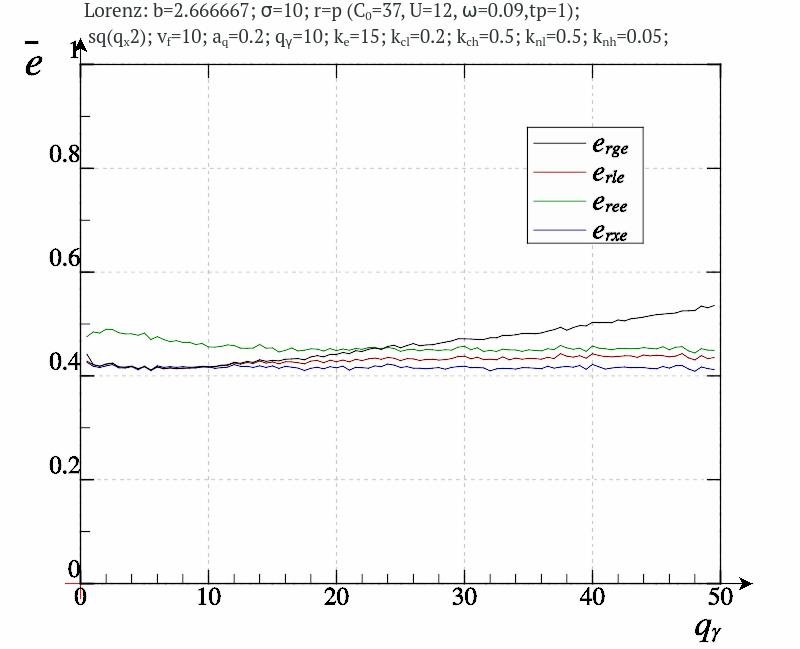
\includegraphics[width=0.49\textwidth]{p/cha/lor/qAuv5.3r/lor_qAuv5_3r_qx2-p_qgamma_e_sign.png}
    \hfill
    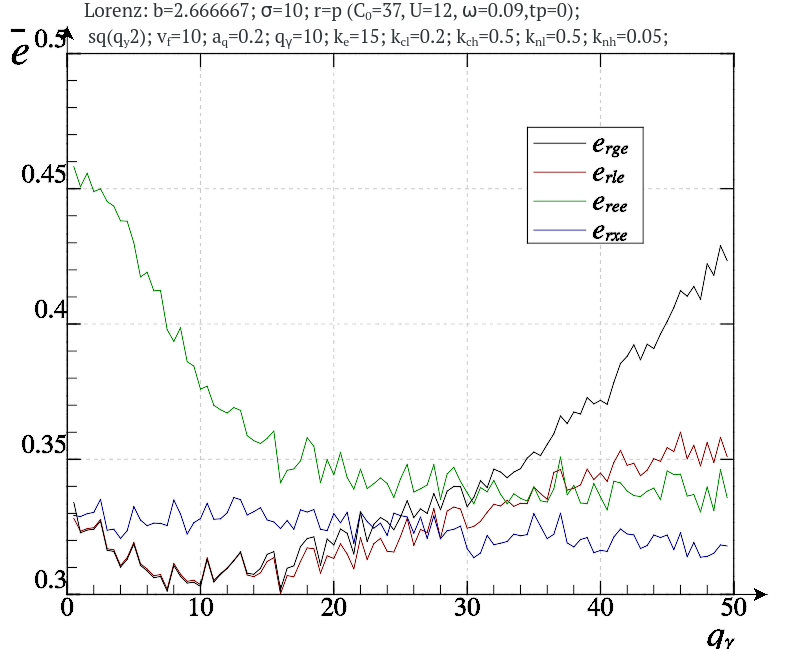
\includegraphics[width=0.49\textwidth]{p/cha/lor/qAuv5.3r/lor_qAuv5_3r_qx2-p_qgamma_e_sin.png}
  }
  \caption{Зависимости $\overline{e}_{r*}(q_\gamma)$ при идентификации системы Лоренца методом qAuv5.3r.$q_{x^2}$
   при~(\ref{atu:eq:lor_po_t_sign}) и (\ref{atu:eq:lor_po_t_sin})}
  \label{atu:f:lor_qg_qAuv5.3r.q_x2}
\end{figure}



На рис.~(\ref{atu:f:lor_qg_qAuv5.3r.q_y2}) представлены зависимости
усреднённых ошибок идентификации системы Лоренца от $q_\gamma$ при использованни метода qAuv5.3r.$q_{y^2}$.
Здесь результаты аналогичны предыдущему случаю. Однако,
данный подход оказалсф более чувствительным к заниженным значением $q_\gamma$.

\begin{figure}[h!]
  \centerline{
    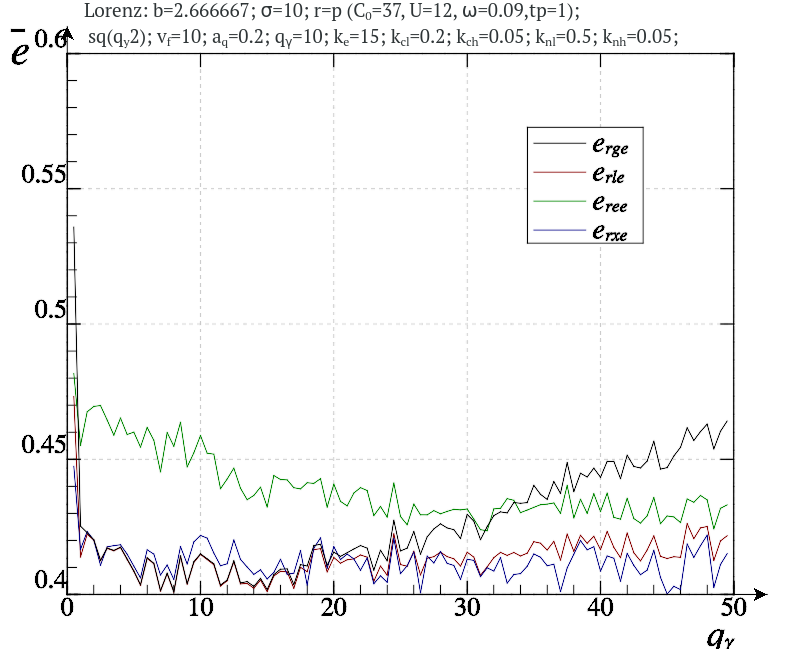
\includegraphics[width=0.49\textwidth]{p/cha/lor/qAuv5.3r/lor_qAuv5_3r_qy2-p_qgamma_e_sign.png}
    \hfill
    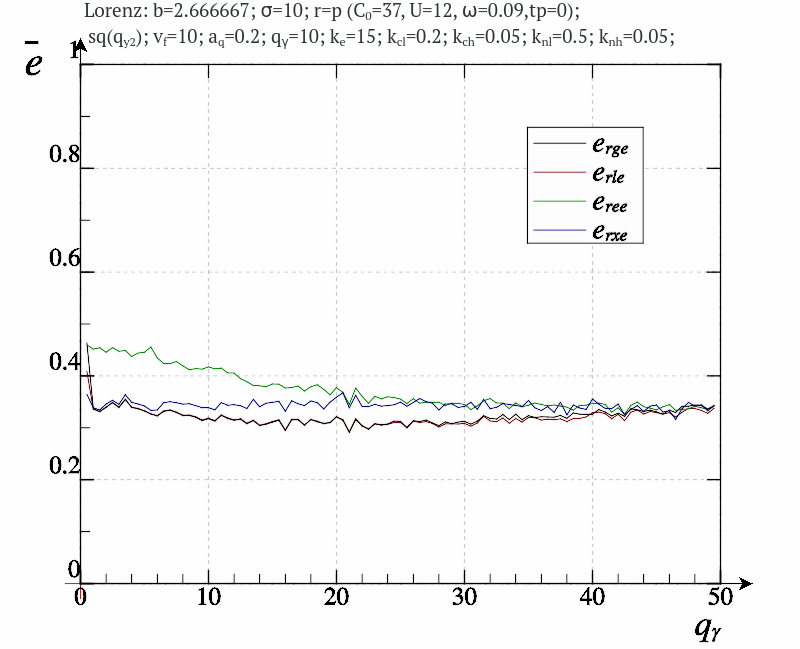
\includegraphics[width=0.49\textwidth]{p/cha/lor/qAuv5.3r/lor_qAuv5_3r_qy2-p_qgamma_e_sin.png}
  }
  \caption{Зависимости $\overline{e}_{r*}(q_\gamma)$ при идентификации системы Лоренца методом qAuv5.3r.$q_{y^2}$
   при~(\ref{atu:eq:lor_po_t_sign}) и (\ref{atu:eq:lor_po_t_sin})}
  \label{atu:f:lor_qg_qAuv5.3r.q_y2}
\end{figure}


На рис.~(\ref{atu:f:lor_qg_FAlv5.3z.q_x2}) представлены зависимости
усреднённых ошибок идентификации системы Лоренца от $q_\gamma$ при использованни метода FAlv.3z.$q_{x^2}$.
В этом случае зависимости сильно отличаются от двух предыдущих случаев.
Так как этот метод непосредственно используют функцию
качества для орпделения $p_e$ каждым агентом, то зависимость
иметт явній єкстремальній характер.
При малых значениях $q_\gamma$ чувствительность избыточна,
и процесс поиска нарушается.
При больших -- недостаточна, и помимо издыточного вляния ``дальних'' агентов также снижается скорость и точность поиска.
Влияние  ``дальних'' агентов игнорируется при использовании
$p_{le}$ и $p_{ee}$, однако,
в эти методы теряются точность при переключении
между лучшими агентами.


\begin{figure}[h!]
  \centerline{
    \includegraphics[width=0.49\textwidth]{p/cha/lor/FAlv5.3z/lor_FAlv5_3z_qx2-p_qg_e_sign.png}
    \hfill
    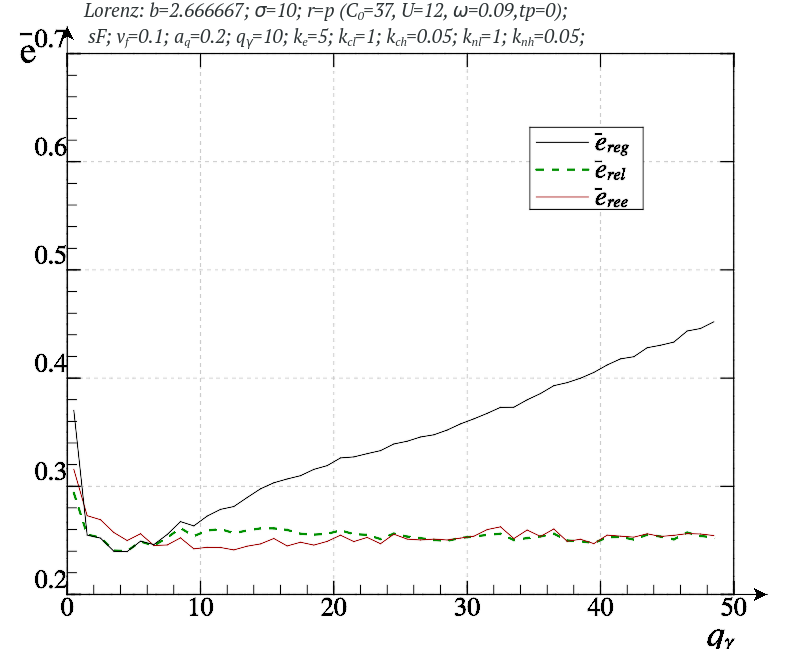
\includegraphics[width=0.49\textwidth]{p/cha/lor/FAlv5.3z/lor_FAlv5_3z_qx2-p_qg_e_sin.png}
  }
  \caption{Зависимости $\overline{e}_{r*}(q_\gamma)$ при идентификации системы Лоренца методом FAlv5.3z.$q_{x^2}$
   при~(\ref{atu:eq:lor_po_t_sign}) и (\ref{atu:eq:lor_po_t_sin})}
  \label{atu:f:lor_qg_FAlv5.3z.q_x2}
\end{figure}


Разультаты моделирования процессов идентификации параметра ``$r$''
системы Лоренца позволяют в целос сделать слкдубщие выводы:





% habr: 
% 1. Конвекция в тороидальной трубе (Ланда П.С. Нелинейные колебания и волны. — М: Либроком, 2010, с. 454-455)
% 2. Одномодовый лазер (Покровский Л.А. Решение системы уравнений Лоренца в
%  асимптотическом пределе большого числа Релея. I. Система Лоренца в простейшей
%  квантовой модели лазера и приложение к ней метода усреднения // Теоретическая
%  и математическая физика, 1985, т. 62, №2, с. 272-290);
% 3. Осциллятор с инерционным возбуждением (Неймарк Ю.И., Ланда П.С.
% Стохастические и хаотические колебания. — М: Либроком, 2009, с. 288-295).
